
\documentclass[8pt]{article}

\usepackage[utf8]{inputenc}

\usepackage{amsmath, bm}
\usepackage{graphicx}
\usepackage{amssymb}
\usepackage{float}
\usepackage{caption}
\usepackage{subcaption}
% set font size to 11pt

% set margin
\usepackage[margin=0.5in]{geometry}

\setlength{\parskip}{\baselineskip}%
\setlength{\parindent}{0pt}%
\setlength{\headsep}{5pt}

\begin{document}

% insert pdf cover page here


\title{Lab report: 3A1 Drag of bluff and streamlined bodies}
\author{lwp26}
\date{November 2023}
\maketitle

\section{Introduction}

The understanding of drag force for various bodies, and flow regimes is crucial to designing efficient transportation in aeronautical and maritime engineering.
In this report, the drag force on a sphere, flat plate and streamlined body is measured and a graph of drag coefficient against Reynolds number is plotted.
The spherical body was tested with and without a turbulence inducing trip wire to investigate the difference.
The flow patterns around the bodies are also visualised using tufts and streamlines.

\section{Method}
Each body was placed in the Markham wind tunnel and 12 measurements of drag were taken at $1$mBar intervals of dynamic pressure differences up to $12$mBar.
A counterweight was used to balance the drag force such that the body remained in the same position. The drag force was a factor of the weight added.

\section{Theory}

\subsection{Dimensionless Quantities}

The flow is taken to be invicid and in the large section before the contraction of the Markham Tunnel, the velocity is negligible, and so the pressure there is the stagnation pressure $p_0$.
\begin{equation}
    p_0 + 0 = p + \frac{1}{2}\rho U^2 \implies U = \sqrt{\frac{2(p_0-p)}{\rho_a}}
    \label{eq1}
\end{equation}
The pressure difference between the large section and working section, $p_0 - p$ is measured by a pressure transducer.
\begin{equation}
    Re = \frac{Ud}{\nu}
    \label{re}
\end{equation}
The drag coefficient is calculated from the drag force, $D$, the frontal area, $S$, and the dynamic pressure.
\begin{equation}
    D = C_d \frac{1}{2} \rho U^2 S \implies C_d = \frac{2D}{ \rho U^2 S}
\end{equation}
The density of air is calculated from measured temperature and pressure using the ideal gas law.
\begin{equation}
    \rho_a = \frac{P}{RT}
\end{equation}

\subsection{Calculated Uncertainty}

Sources of uncertainty in calculating Reynolds number in equation \ref{re} is shown below.
\begin{equation}
    u(Re) = u(U) + u(d) + u(\nu)
\end{equation}
The relative uncertainties, $u(D)$ and $u(\nu)$ are negligible compared to $u(U)$ as the diameter was measured to a higher degree of precision and the viscosity change for the uncertainty in measured temperature is also negligible.
\begin{equation}
    u(Re) \approx u(U) = \frac{1}{2}u(p_0-p) + \frac{1}{2}u(\rho_a)
    \label{eq5}
\end{equation}
From considering uncertainty from ideal gas law, .
\begin{equation}
     u(\rho_a) = u(T) + u(P)
\end{equation}

Sources of uncertainty in $C_d$, taking $S=\pi d^2/4$.
\begin{equation}
    u(C_d) = u(D) + u(\rho_a U^2) + u(S) = u(D) + u(\frac{1}{2}\rho_a U^2) + 2u(d)
\end{equation}
Substituting equation \ref{eq1} and same reasoning as for equation \ref{eq5} that $u(d)$ is negligible.
\begin{equation}
    u(C_d) \approx u(D) + u(p_0-p)
\end{equation}


\subsection{Measurement Uncertainty}
The measurement of dynamic pressure, $p_0-p$, was done with a calibrated pressure sensor, and so the source of absolute uncertainty is taken at the 2 decimal point precision of the sensor.

The uncertainty in drag reading is harder to quantify, as it was observed to fluctuate at higher speeds.
The setup involved buckets of oil to dampen the fluctuations in the drag force, but this was not completely effective.
Single point measurements were taken at each speed, and so the standard deviation of the drag reading is not known.
Instead the uncertainty in the drag reading is taken to be at the 1 point decimal precision, which is valid at low speeds where the drag reading is stable.
The uncertainty in the correction factor to convert the reading into Newtons is taken to be 0.

The Temperature was measured with a temperature gauge with a precision of $1^oC$, this may seem crude, however, on conversion to Kelvin this gives a small relative uncertainty.

The pressure was measured in inches of mercury, with a very high precision of $0.001$ inches.
Changes in mercury's density for the small temperature changes are also negligible and so the atmospheric pressure has negligible uncertainty.



\section{Discussion}

% 1. Discuss the observations and measurements of the forces and flow fields around the three bodies. Sketch the flow patterns.

The drag force was observed to increase with increasing dynamic pressure, as expected.
Temperature was observed to increase in the tunnel by $3^oC$ over the course of the experiment, which was accounted for in the calculation of air density.
This is caused by the recycled air in the Markham tunnel being heated by the fan compression.

The flow patterns around the bodies were visualised using tufts which are parallel to the streamlines.
These can be seen in figures \ref{fig:figure4}, \ref{fig:figure6} and \ref{fig:figure10} for the flat plate, sphere and streamlined body respectively.
Figure 


Figure \ref{fig:figure1} shows the plot of drag coefficient, $C_d$ vs Reynolds number, $Re_D$ for the various bodies. 
For the sphere, the critical Reynolds number where the drag coefficient rapidly decreases is marked on the graph.
This is due to seperation occuring behind the maximum circumference shoulder and so the size of the size of the wake is reduced.
This was further demonstrated by spraying parafin oil on the sphere and observing where the oil collected on the surface.
Photos of the seperation point at low and high Reynolds number are shown in figures \ref{fig:figure2} and \ref{fig:figure3} respectively.

The error in the drag coefficient is plotted as a transparent band on the graph.
This is however only visible at low Reynolds number, as relative uncertainty is larger at smaller dynamic pressures.
The true uncertainty is likely to increase at higher Reynolds number due to the increased fluctuations in the drag reading, not accounted for in the uncertainty analysis.

This reduction in wake significantly reduces the pressure drag.
It can also be seen that the sphere with trip wire has a lower drag coefficient at smaller reynolds numbers.
This is because the trip wire causes the boundary layer to become turbulent, and so the boundary layer is turbulent for longer, reducing the size of the wake and hence the pressure drag.

% 4. Estimate the errors in the drag coefficients at the lowest speed for all the bodies and mark on your graph. Is the error in the drag coefficient constant? You must include any equations you use to estimate errors in your report.

% This is done in the uncertainty section

% 5. Explain the difference in the Cd versus Reynolds number curves for the different bodies in terms of the flow patterns and the different contributions of form and skin-friction drag.

The various bodies have different contributions of form and skin friction drag.

The flat plate has the smallest wetted area, and the largest wake. The wake is larger than the frontal area, leading to a drag coefficient greater than 1.
This suggests that the form drag is significantly greater than the skin friction drag for the flat plate.

The sphere in low Reynolds number flow, seperation occurs before the shoulder and so the wake area is slightly larger than the frontal area.
The wetted area is larger than the flat plate, however the form drag is still the significant contributor to the total drag.

Considering the tripped sphere where seperation occurs after the shoulder, the wake area is smaller than the frontal area and so the form drag is reduced.
The skin friction drag is increased both due to an increase in wetted area and the now turbulent boundary layer.
Skin friction drag of a turbulent boundary layer is greater than laminar boundary layer due to an increased velocity gradient at the surface as seen in the IB Boundary Layer lab.
Both of these effects contribute to the total drag coefficient.
A rather interesting observation is that as the drag coefficient of the tripped sphere, increases above that of the untripped sphere at higher Reynolds number.
This may be due to the larger turbulent boundary layer of the tripped sphere, as the position of the trip wire is before the shoulder.
However, this is not conclusive due to the fluctuations in drag measurements at higher Reynolds numbers.

Streamlined body has the largest wetted area, and a negligible wake area giving it the smallest drag coefficient of the bodies. 
This suggests that the skin friction drag is the significant contributor to the total drag.

% 6. Explain what is meant by fineness ratio and why there is an optimum for a “streamlined body”.

The fineness ratio is the ratio of the length of the body to the diameter of the body.

The form drag is proportional to frontal area and skin friction drag is proportional to wetted area.
The optimum fineness ratio is at the minimum wetted area such that seperation occurs at the end of the body.
This minimises the form drag and skin friction drag, giving the minimum total drag coefficient.



\begin{figure}[H]
    \centering
    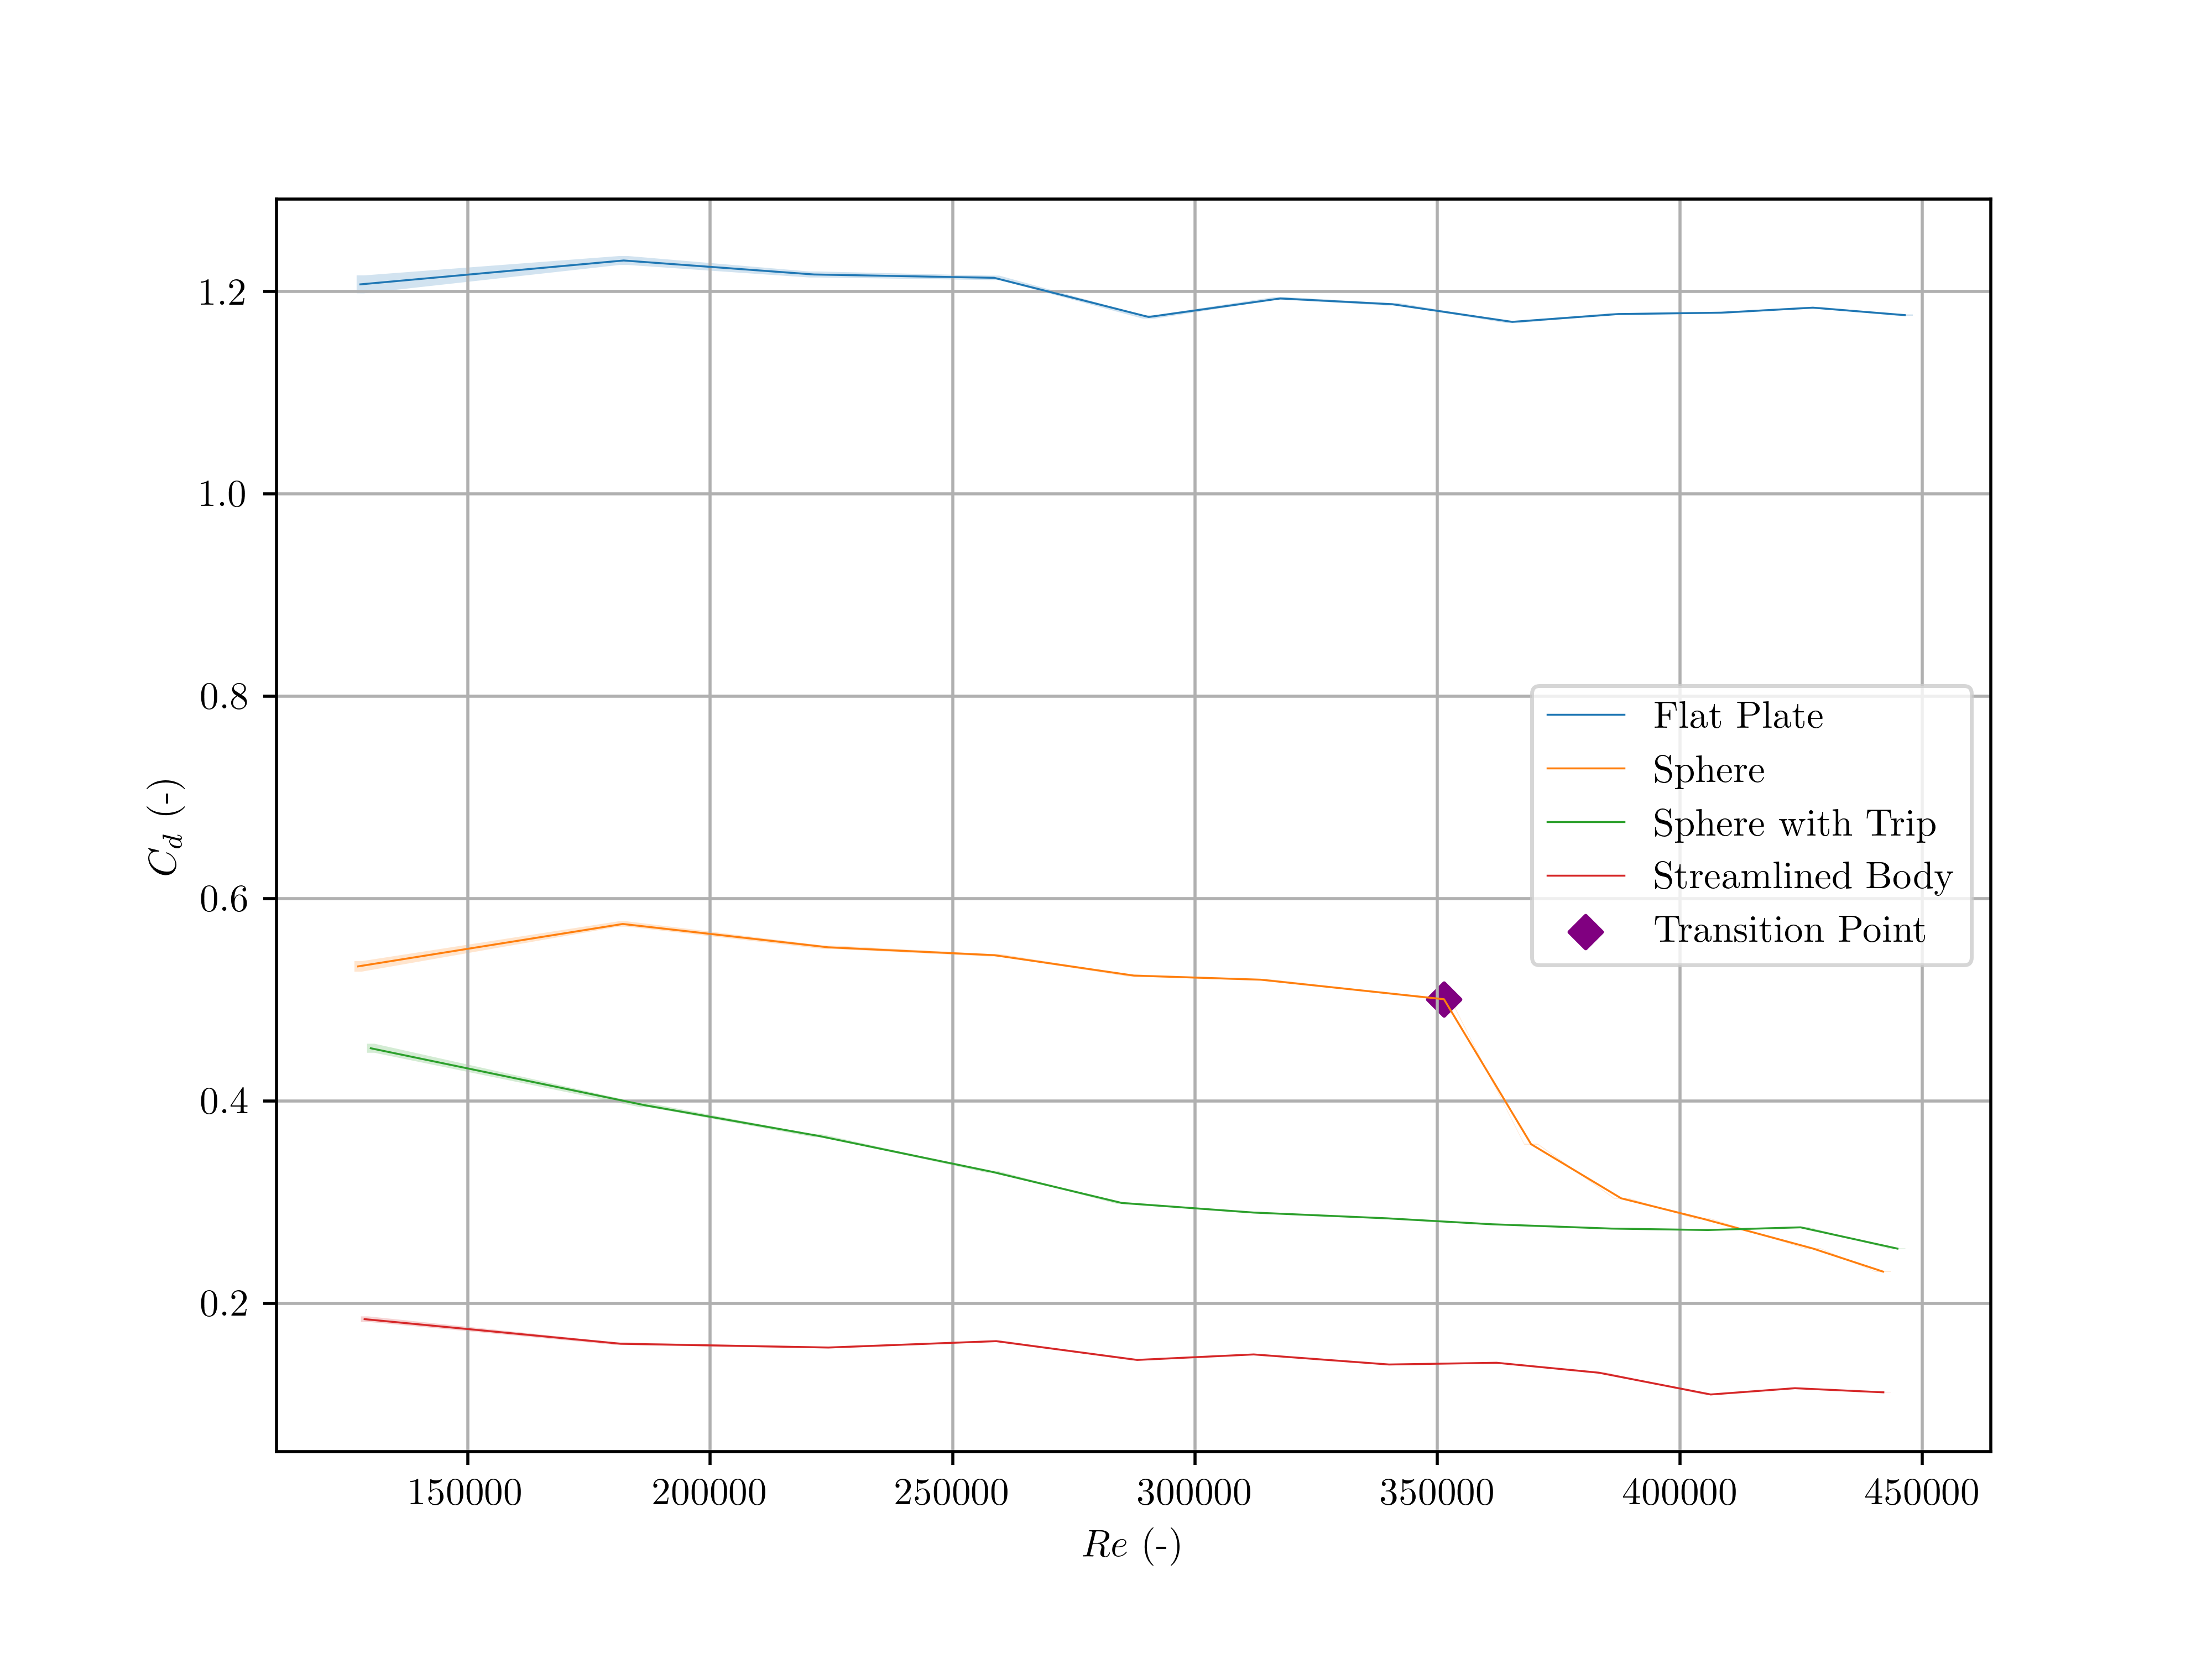
\includegraphics[width=0.8\textwidth]{Re_vs_Cd.png}
    \caption{Graph of drag coefficient against Reynolds number for various bodies}
    \label{fig:figure1}
\end{figure}

\begin{figure}[H]
    \centering
    \begin{subfigure}[t]{0.48\textwidth}
        \centering
        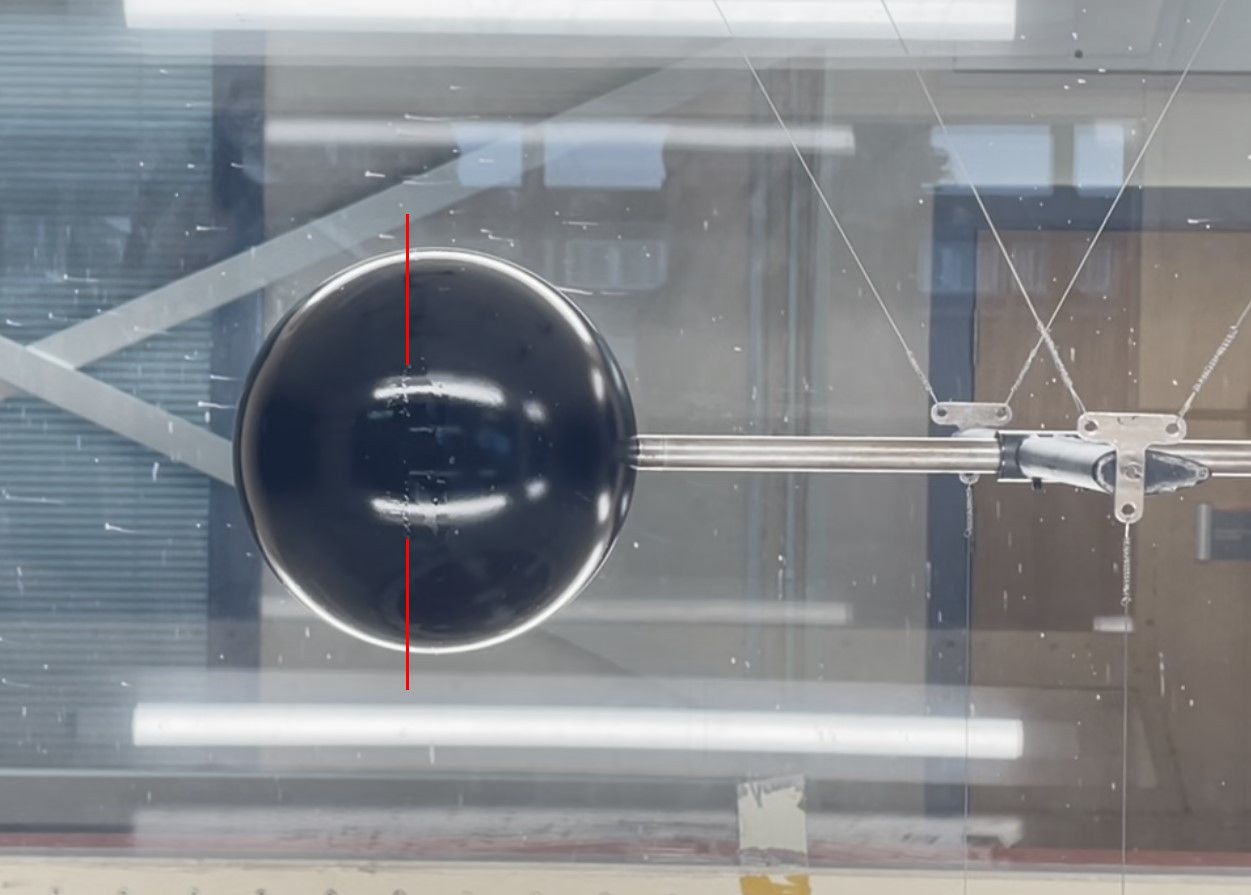
\includegraphics[width=1\textwidth]{Images_Videos/early_seperation_annotated.jpg}
        \caption{Seperation before shoulder}
        \label{fig:figure2}
    \end{subfigure}
    ~
    \begin{subfigure}[t]{0.48\textwidth}
        \centering
        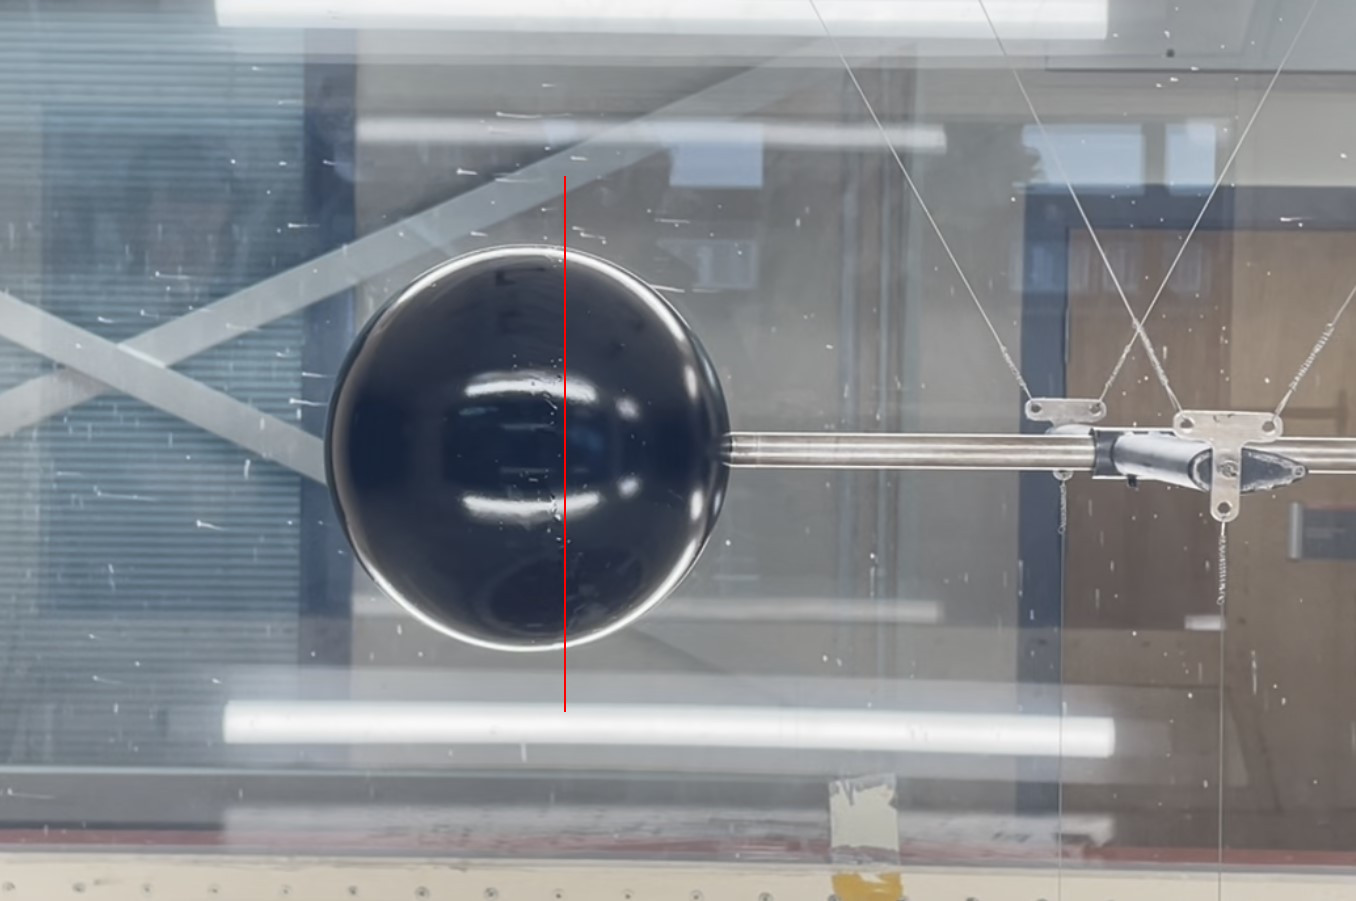
\includegraphics[width=1\textwidth]{Images_Videos/late_seperation_annotated.jpg}
        \caption{Seperation after shoulder at higher Re}
        \label{fig:figure3}
    \end{subfigure}
\end{figure}

\begin{figure}[H]
    \centering
    \begin{subfigure}[t]{0.48\textwidth}
        \centering
        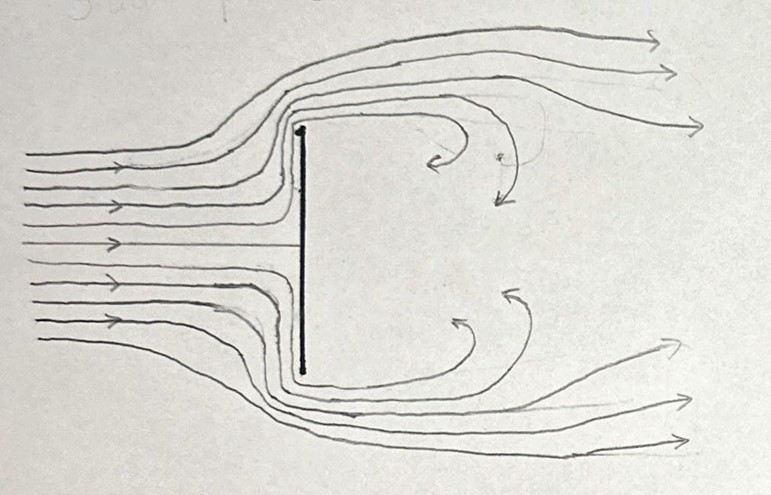
\includegraphics[width=1\textwidth]{Images_Videos/stream_flat_plate_1.jpg}
        \caption{Streamline drawing}
        \label{fig:figure4}
    \end{subfigure}
    ~
    \begin{subfigure}[t]{0.48\textwidth}
        \centering
        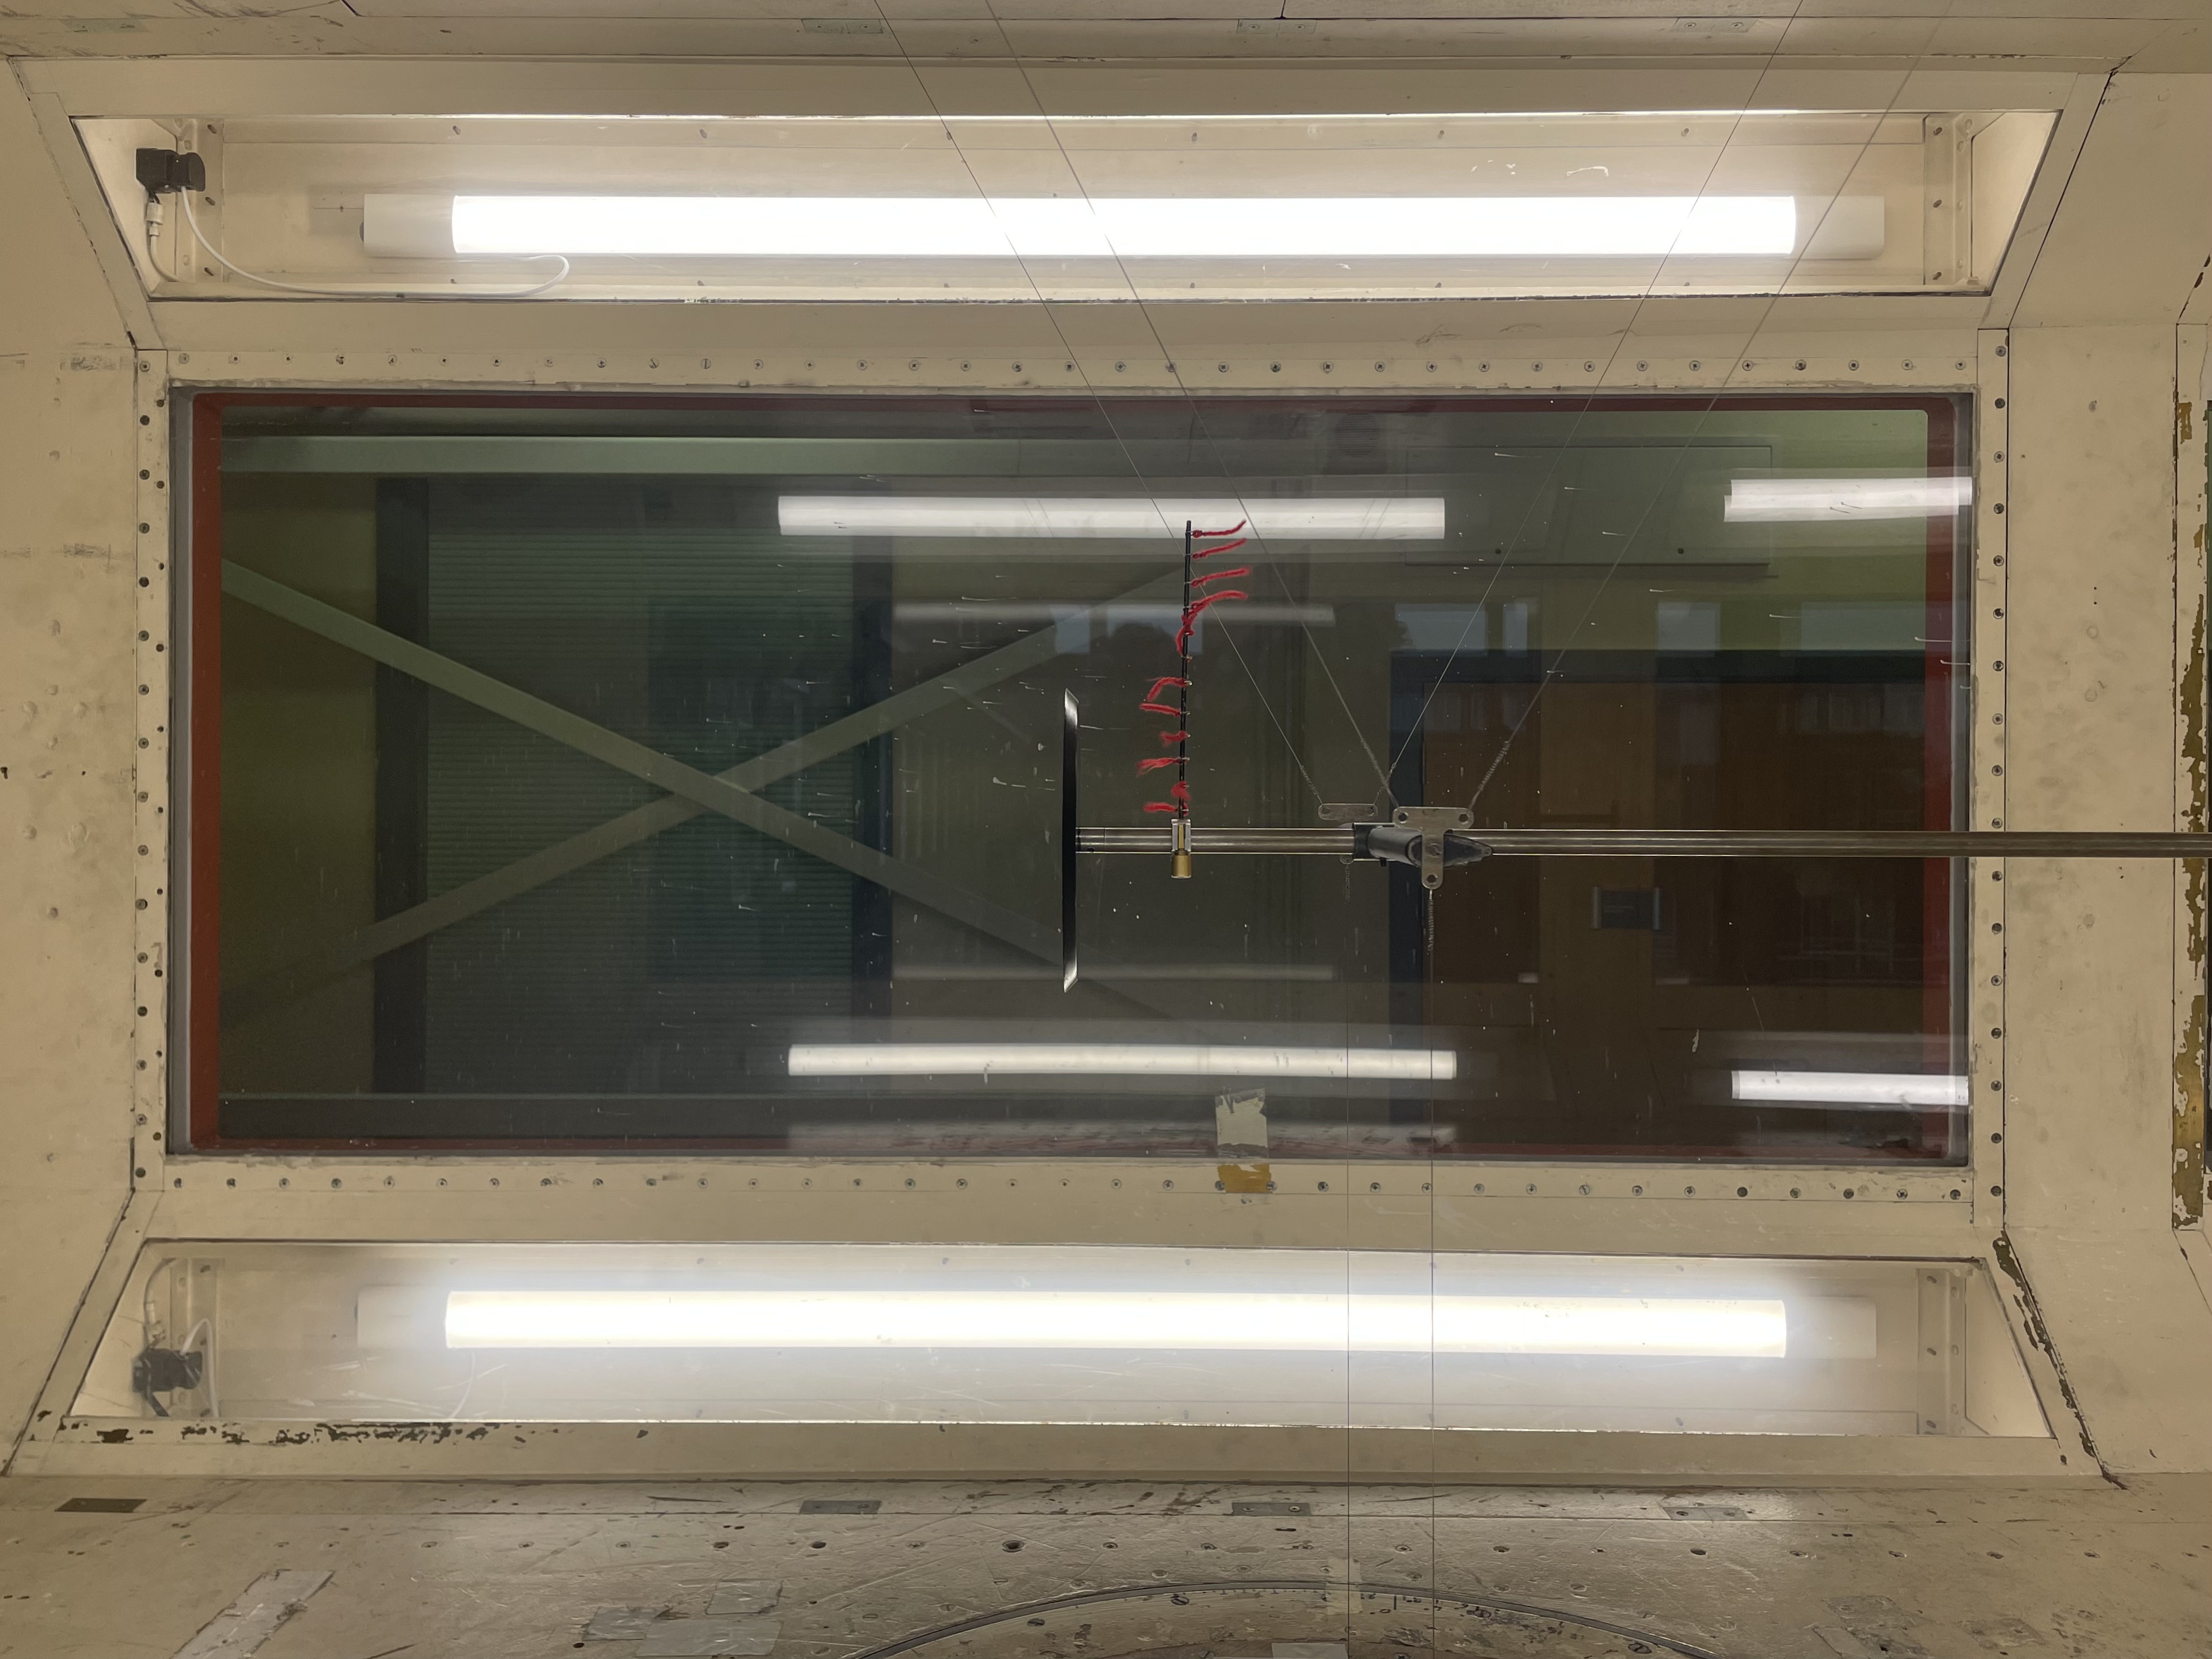
\includegraphics[width=1\textwidth]{Images_Videos/Plate_8milibar.jpg}
        \caption{Tuft visualisation}
        \label{fig:figure5}
    \end{subfigure}
    \caption{Streamlines and tuft visualisation for flat plate}
\end{figure}

\begin{figure}[H]
    \centering
    \begin{subfigure}[t]{0.48\textwidth}
        \centering
        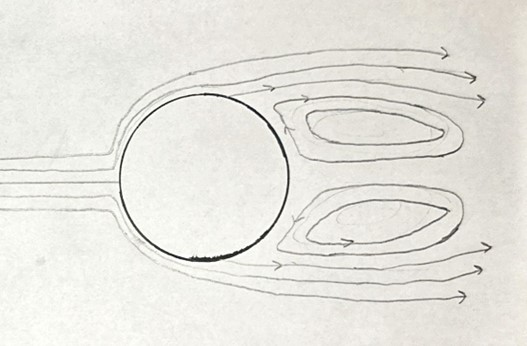
\includegraphics[width=1\textwidth]{Images_Videos/stream_low_Re_sphere.jpg}
        \caption{Streamline drawing}
        \label{fig:figure6}
    \end{subfigure}
    ~
    \begin{subfigure}[t]{0.48\textwidth}
        \centering
        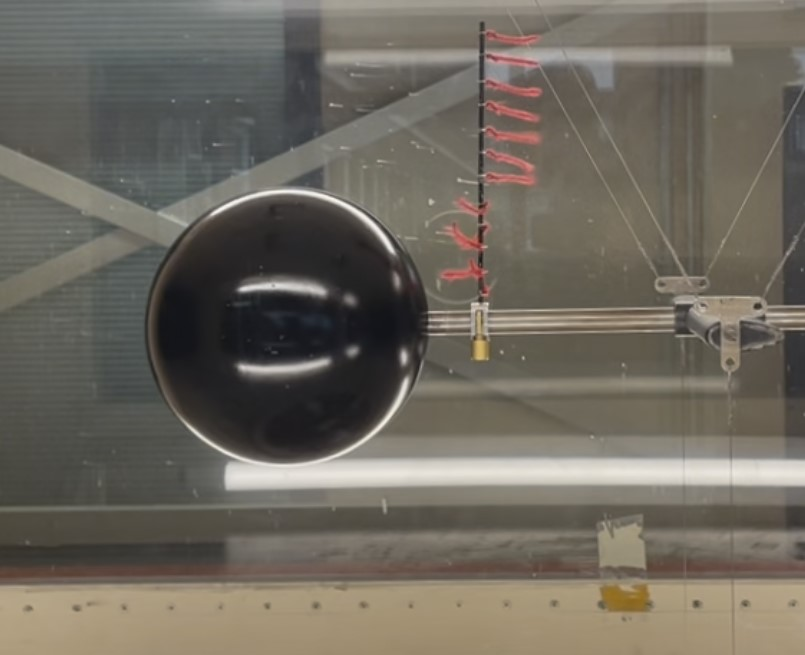
\includegraphics[width=1\textwidth]{Images_Videos/sphere_low_Re.jpg}
        \caption{Tuft visualisation}
        \label{fig:figure7}
    \end{subfigure}
    \caption{Streamlines and tuft visualisation for sphere at low Reynolds number}
\end{figure}

\begin{figure}[H]
    \centering
    \begin{subfigure}[t]{0.48\textwidth}
        \centering
        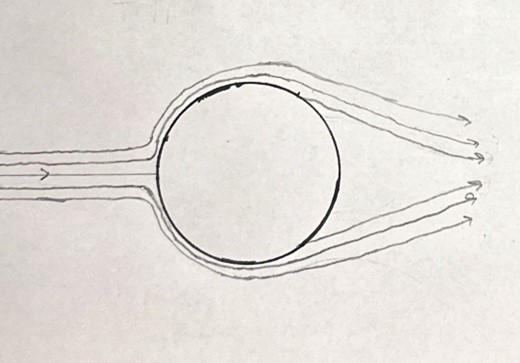
\includegraphics[width=1\textwidth]{Images_Videos/stream_hi_Re_sphere.jpg}
        \caption{Streamline drawing}
        \label{fig:figure8}
    \end{subfigure}
    ~
    \begin{subfigure}[t]{0.48\textwidth}
        \centering
        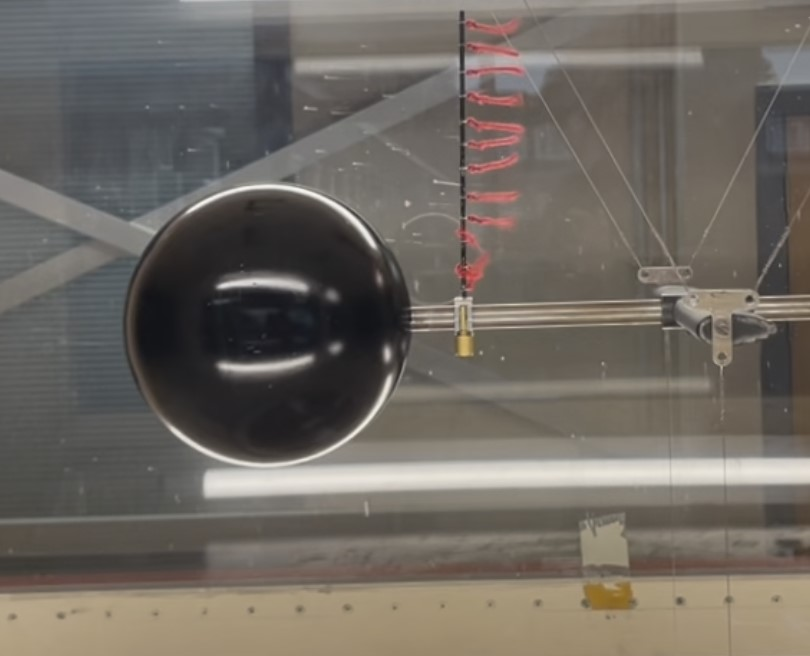
\includegraphics[width=1\textwidth]{Images_Videos/sphere_high_Re.jpg}
        \caption{Tuft visualisation}
        \label{fig:figure9}
    \end{subfigure}
    \caption{Streamlines and tuft visualisation for sphere at high Reynolds number}
\end{figure}

\begin{figure}[H]
    \centering
    \begin{subfigure}[t]{0.48\textwidth}
        \centering
        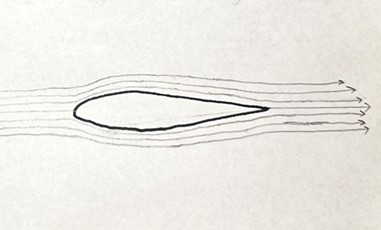
\includegraphics[width=1\textwidth]{Images_Videos/stream_streamlined.jpg}
        \caption{Seperation before shoulder}
        \label{fig:figure10}
    \end{subfigure}
    ~
    \begin{subfigure}[t]{0.48\textwidth}
        \centering
        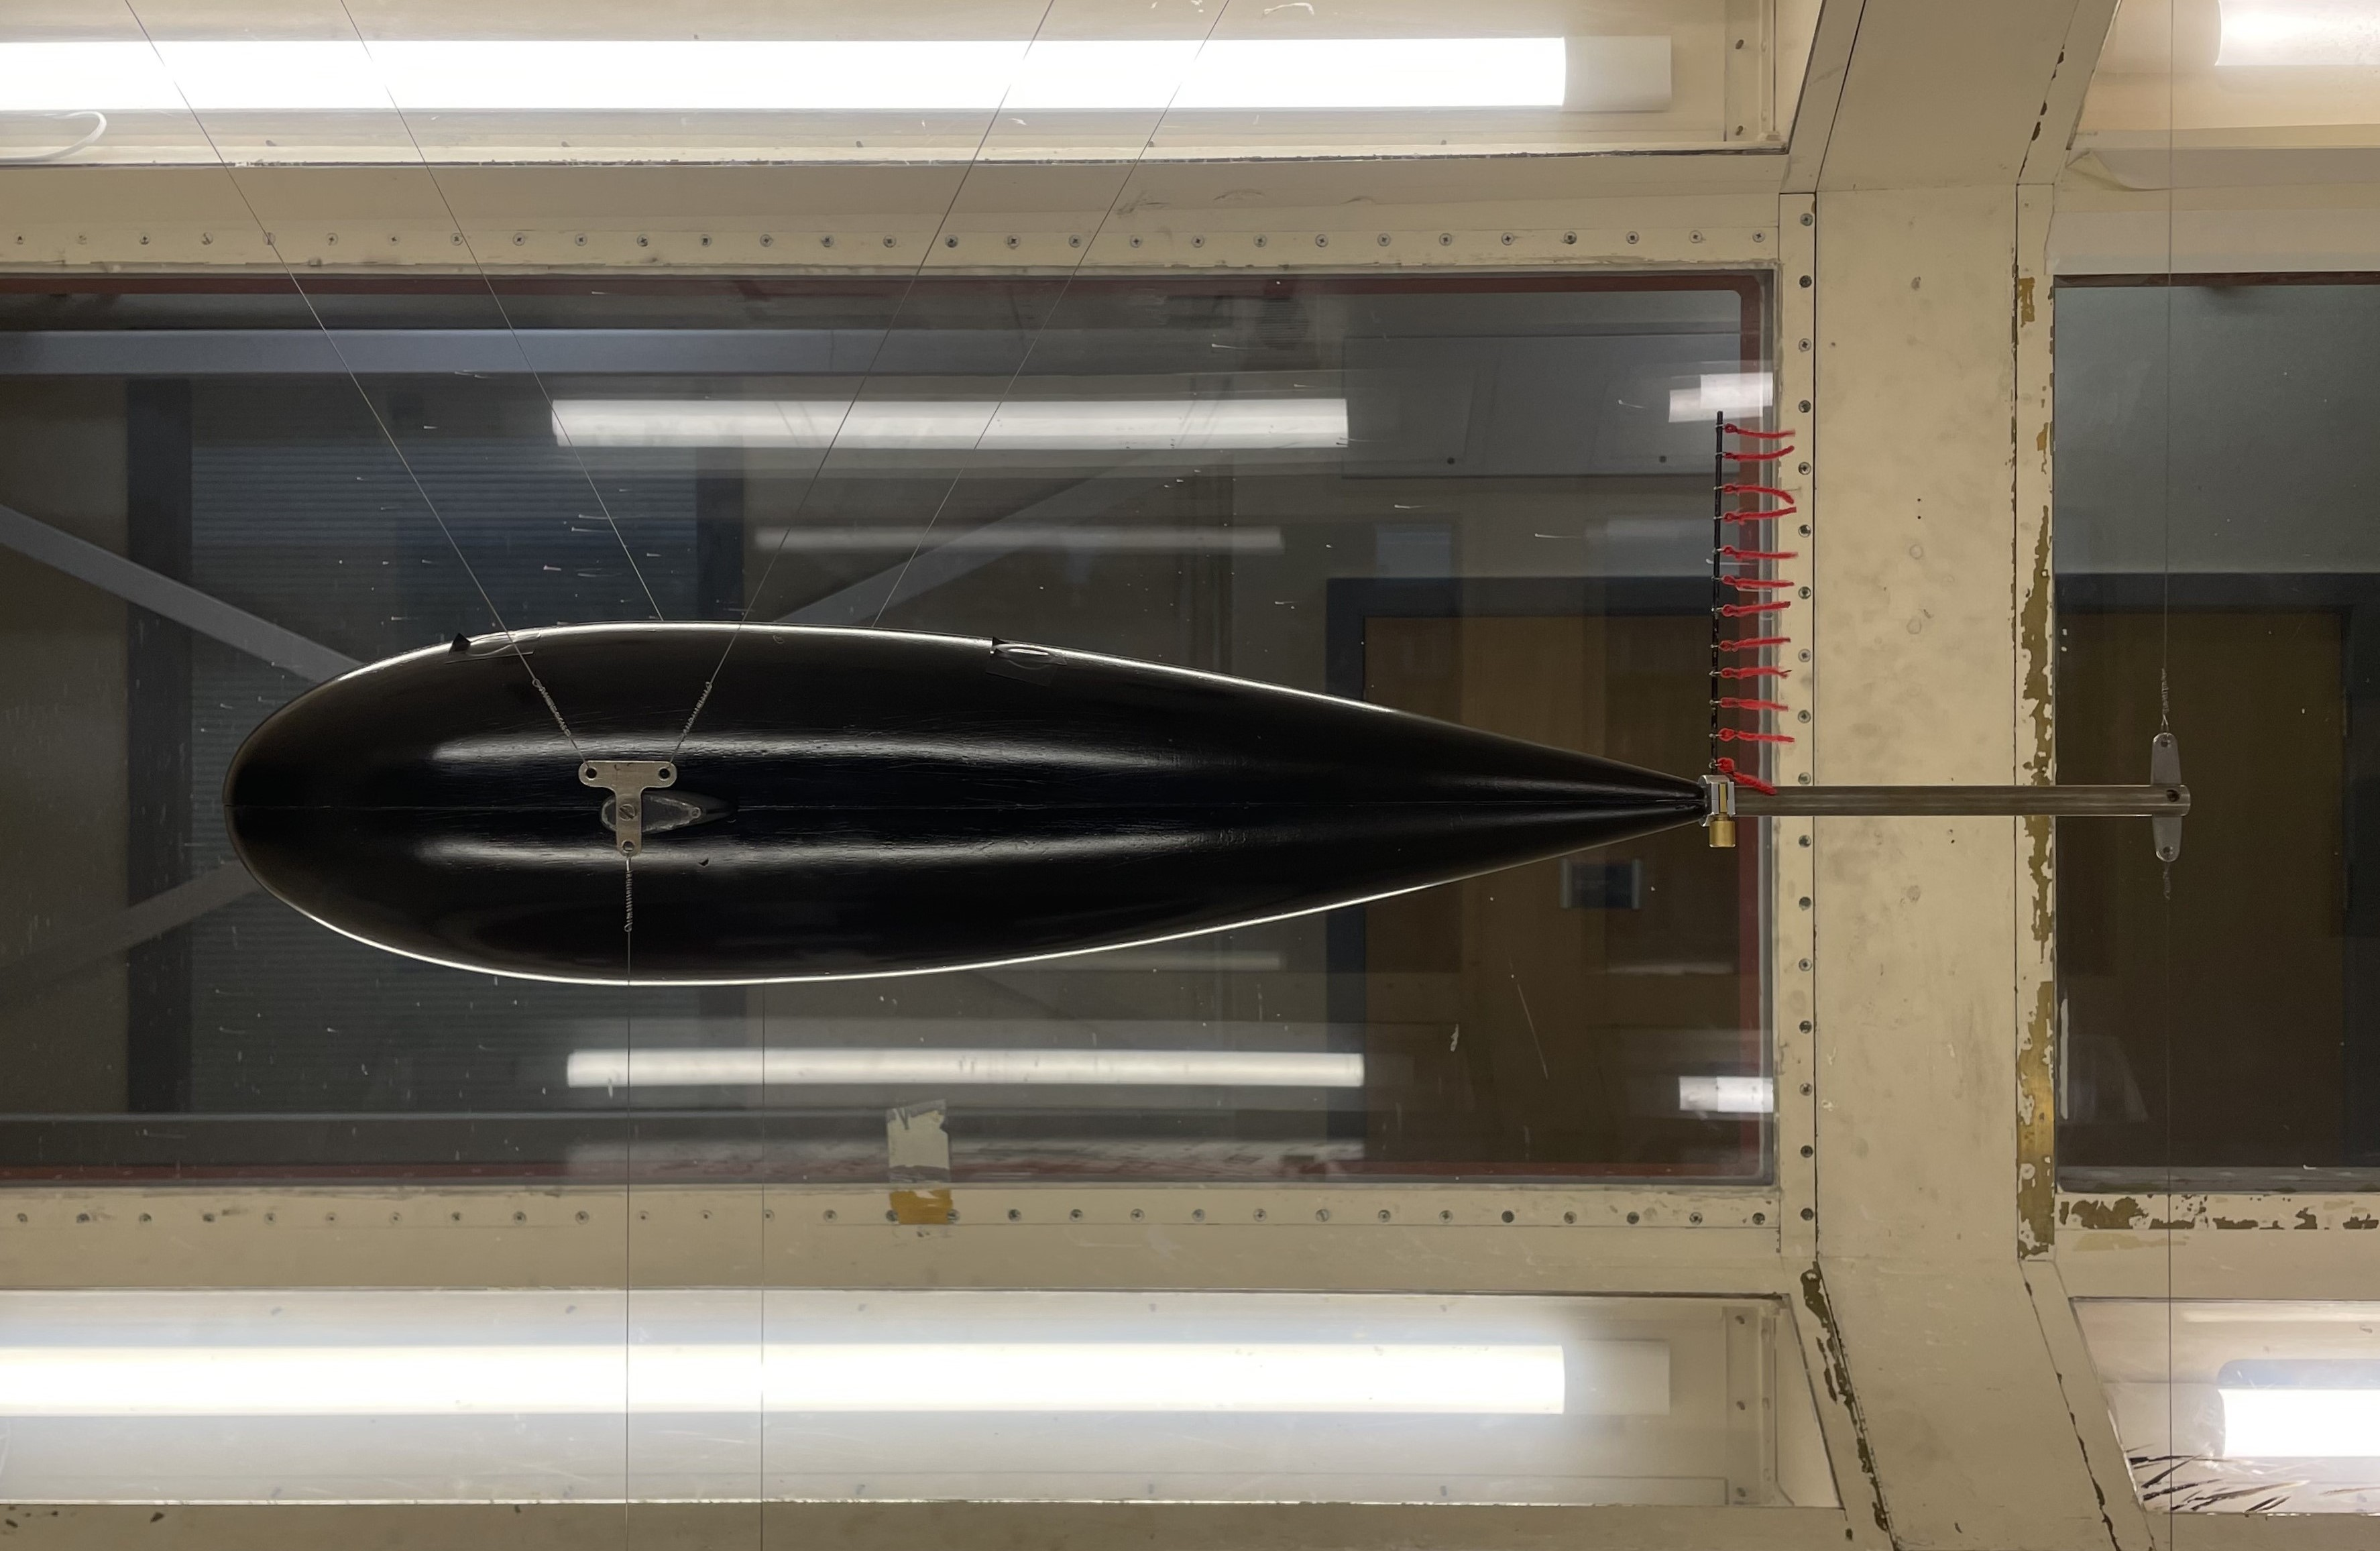
\includegraphics[width=1\textwidth]{Images_Videos/Streamlined_8milibar.JPG}
        \caption{Seperation after shoulder at higher Re}
        \label{fig:figure11}
    \end{subfigure}
    \caption{Streamlines and tuft visualisation for streamlined body}
\end{figure}

\end{document}
